% Opsætter KU Tex dokument
%%%%%%%%%%%%%%%%%%%%%%%%%%%%%%%%%%%%%%%%%%%%%%%%%%%%%%%%%%%%%%%%%%%%%%%%%%%%%%%%
\documentclass{article}                                                        %
\usepackage[a4paper, hmargin={2.8cm, 2.8cm}, vmargin={2.5cm, 2.5cm}]{geometry} %
\usepackage{eso-pic}  % \AddToShipoutPicture                                   %
\usepackage{graphicx} % \includegraphics                                       %
\usepackage{subfig}    
\usepackage{setspace}                                                        %
%%%%%%%%%%%%%%%%%%%%%%%%%%%%%%%%%%%%%%%%%%%%%%%%%%%%%%%%%%%%%%%%%%%%%%%%%%%%%%%%

% Pakker til skrifttyper, tekst osv.
%%%%%%%%%%%%%%%%%%%%%%%%%%%%%%%%%%%%%%%%%%%%%%%%%%%%%%%%%%%%%%%%%%%%%%%%%%%%%%%%
    \usepackage[utf8]{inputenc}  % Implementere Unicode                        %
    \usepackage[T1]{fontenc}     % Unicode skrifttype fx. é skrives som 1 tegn %
    \usepackage[english]{babel}   % Dansk Ordbog                                %
    \usepackage{microtype}       % Forbedre linjeombrydningen                  %
    \usepackage{libertine}       % Skrifttype                                  %
%%%%%%%%%%%%%%%%%%%%%%%%%%%%%%%%%%%%%%%%%%%%%%%%%%%%%%%%%%%%%%%%%%%%%%%%%%%%%%%%

% Pakker til matematik og kode.
%%%%%%%%%%%%%%%%%%%%%%%%%%%%%%%%%%%%%%%%%%%%%%%%%%%%%%%%%%%%%%%%%%%%%%%%%%%%%%%%
    \usepackage{mathtools}       % Udvidelse til amsmath pakken                %
    \usepackage{amsthm}          % Pakke til bevisførelse                      %
    \usepackage{amssymb}         % Extra matematiske symboler                  %				
	\usepackage{mychemistry}												   %
	\usepackage[version=3]{mhchem}											   %
	\usepackage{wrapfig}													   %
	\usepackage{siunitx}	
	\usepackage{anyfontsize}
	\usepackage{url}
	\usepackage{ragged2e}
	\usepackage{algorithm2e}
	\usepackage[final]{pdfpages}
	\usepackage{listings}
	\usepackage{todonotes}

	\definecolor{light-gray}{gray}{0.85}
	\definecolor{dkgreen}{RGB}{0.0,128.0,43.0}
	\lstdefinelanguage{FSharp}%
{morekeywords={let, new, match, with, rec, open, module, namespace, type, of, member, % 
and, for, while, true, false, in, do, begin, end, fun, function, return, yield, try, %
mutable, if, then, else, cloud, async, static, use, abstract, interface, inherit, finally, int },
  otherkeywords={ let!, return!, do!, yield!, use!, var, from, select, where, order, by },
  keywordstyle=\color{bluekeywords},
  sensitive=true,
  basicstyle=\ttfamily,
	breaklines=true,
  xleftmargin=\parindent,
  aboveskip=\bigskipamount,
	tabsize=4,
  morecomment=[l][\color{dkgreen}]{///},
  morecomment=[l][\color{dkgreen}]{//},
  morecomment=[s][\color{dkgreen}]{{(*}{*)}},
  morestring=[b]",
  showstringspaces=false,
  literate={`}{\`}1,
  stringstyle=\color{redstrings},
}
	
	\lstset{frame=tb,
  	language=FSharp,			%CHANGE LANGUAGE
  	aboveskip=3mm,
  	belowskip=3mm,
  	showstringspaces=false,
  	columns=flexible,
  	basicstyle={\small\ttfamily},
  	numbers=none,
  	numberstyle=\tiny\color{gray},
  	keywordstyle=\color{blue},
  	commentstyle=\color{dkgreen},
  	stringstyle=\color{mauve},
  	breaklines=true,
  	breakatwhitespace=true,
  	tabsize=3,
  	backgroundcolor=\color{light-gray},
	}
												   %
%%%%%%%%%%%%%%%%%%%%%%%%%%%%%%%%%%%%%%%%%%%%%%%%%%%%%%%%%%%%%%%%%%%%%%%%%%%%%%%%

% Pakker til layout.
%%%%%%%%%%%%%%%%%%%%%%%%%%%%%%%%%%%%%%%%%%%%%%%%%%%%%%%%%%%%%%%%%%%%%%%%%%%%%%%%
    \usepackage{fancyhdr}            % Gør det muligt at bruge sidehoveder     %
    \usepackage{graphicx}            % Mulighed for bl.a. \includegraphics     %
    \usepackage{colortbl}            % Hvis man vil farvelægge sine tabeller   %
    \usepackage{array}               % Gør miljøerne array og tabular bedre    %
    \usepackage{parskip}             % Første paragraf i afsnit indrykkes ikke %
    \usepackage{titlesec}            % Tilpassing af afstand mellem sektioner  %
    \usepackage[lastpage,user]{zref} % Side x af y                             %
%%%%%%%%%%%%%%%%%%%%%%%%%%%%%%%%%%%%%%%%%%%%%%%%%%%%%%%%%%%%%%%%%%%%%%%%%%%%%%%%


% Implementerer en række makroer og de pakker der er importeret
%%%%%%%%%%%%%%%%%%%%%%%%%%%%%%%%%%%%%%%%%%%%%%%%%%%%%%%%%%%%%%%%%%%%%%%%%%%%%%%%
    \pagestyle{fancy}                        % Implementerer sidehoved         %
    \lhead{Københavns Universitet}                % Venstre sidehoved               %
    \rhead{Casper Bresdahl, Torben Milhøj}                             % Højre sidehoved      %
    \cfoot{\thepage\ of \zpageref{LastPage}} % Side x af y                     %
    \newtheorem*{prp}{Propostion}            % Skaber nyt theorem  
    \renewcommand{\baselinestretch}{1.5}       %
%%%%%%%%%%%%%%%%%%%%%%%%%%%%%%%%%%%%%%%%%%%%%%%%%%%%%%%%%%%%%%%%%%%%%%%%%%%%%%%%

% Mindsker afstanden mellem sektioner
%%%%%%%%%%%%%%%%%%%%%%%%%%%%%%%%%%%%%%%%%%%%%%%%%%%%%%%%%%%%%%%%%%%%%%%%%%%%%%%%%%
\titlespacing\section{0pt}{12pt plus 4pt minus 2pt}{0pt plus 1pt minus 3pt}      %
\titlespacing\subsection{0pt}{12pt plus 4pt minus 2pt}{0pt plus 1pt minus 3pt}   %
\titlespacing\subsubsection{0pt}{12pt plus 4pt minus 2pt}{0pt plus 1pt minus 3pt}%
%%%%%%%%%%%%%%%%%%%%%%%%%%%%%%%%%%%%%%%%%%%%%%%%%%%%%%%%%%%%%%%%%%%%%%%%%%%%%%%%%%

%%%%%%%%%%%%
% Document %
%%%%%%%%%%%%

\begin{document}

\begin{titlepage}

\newcommand{\HRule}{\rule{\linewidth}{0.5mm}} % Defines a new command for the horizontal lines, change thickness here

\begin{center}
 % Center everything on the page
 
%----------------------------------------------------------------------------------------
%	HEADING SECTIONS
%----------------------------------------------------------------------------------------

\textsc{\LARGE University of Copenhagen}\\[1.5cm] % Name of your university/college
\textsc{\Large Computer Science}\\[0.5cm] % Major heading such as course name
\textsc{\large Implementation of programming languages}\\[0.5cm] % Minor heading such as course title

%----------------------------------------------------------------------------------------
%	TITLE SECTION
%----------------------------------------------------------------------------------------

\HRule \\[0.4cm]
{ \huge \bfseries Fasto Compiler}\\[0.4cm] % Title of your document
\HRule \\[1.5cm]
 
%----------------------------------------------------------------------------------------
%	AUTHOR SECTION
%----------------------------------------------------------------------------------------

\begin{minipage}{0.4\textwidth}
\begin{flushleft} \large
\emph{Authors:}\\ 
% Your name
Casper \textsc{Bresdahl}\\
Torben \textsc{Milhøj}\\
\end{flushleft}
\end{minipage}
~
\begin{minipage}{0.4\textwidth}
\begin{flushright} \large
\emph{Teachers:} \\
Cosmin \textsc{Oancea}\\
Andrzej \textsc{Filinski}\\
\end{flushright}
\end{minipage}\\[2cm]

% If you don't want a supervisor, uncomment the two lines below and remove the section above
%\Large \emph{Forfattere:}\\
%Axel \textsc{Christof}\\% Your name
%Casper \textsc{Bresdahl}\\
%Emilie \textsc{Bentsen}\\[1cm] 

%----------------------------------------------------------------------------------------
%	DATE SECTION
%----------------------------------------------------------------------------------------

{\large \today}\\[2cm] % Date, change the \today to a set date if you want to be precise

%----------------------------------------------------------------------------------------
%	LOGO SECTION
%----------------------------------------------------------------------------------------


\includegraphics{logo.png}\\[1cm] % Include a department/university logo - this will require the graphicx package
 
%----------------------------------------------------------------------------------------

\vfill % Fill the rest of the page with whitespace

%Disse linjer skaber forside, evt indholdsfortegnelse, og sætter sidetal
%%%%%%%%%%%%%%%%%%%%%%%%%%%%%%%%%%%%%%%%%%%%%%%%%%%%%%%%%%%%%%%%%%%%%%%%%%%%%%%%
									                                           %
    \thispagestyle{empty}   % Fjerner sidetal forside                          %
        % Slå disse til hvis der ønskes indholdsfortegnelse                    %
        %%%%%%%%%%%%%%%%%%%%%%%%%%%%%%%%%%%%%%%%%%%%%%%%%%%%%%%%%%%%%%%%%%%%%%%%
           % TODO2 Hvorfor skal den køres to gange?   
            \newpage                % Side til indholdsfortegnelse            %
            \thispagestyle{empty}   % Fjerner sidetal fra indholdsfortegnelse %
            \tableofcontents        % Skaber indholdsfortegnelse              %
    \end{center}
        %%%%%%%%%%%%%%%%%%%%%%%%%%%%%%%%%%%%%%%%%%%%%%%%%%%%%%%%%%%%%%%%%%%%%%%%
    \newpage                % Første rigtige side
    \setcounter{page}{1}    % Sætter rigtigt sidetal på første side
%%%%%%%%%%%%%%%%%%%%%%%%%%%%%%%%%%%%%%%%%%%%%%%%%%%%%%%%%%%%%%%%%%%%%%%%%%%%%

\end{titlepage}
{\fontsize{12}{14}\selectfont
    \section{Lexer}
The handed out Lexer has been extended as to acommodate for other operators, the implementation of which has also been made elsewhere.
The purpose of the lexer is to recognize our input and "parse" properly to the parser, such that input be distinguished and handled properly.\\
The lexer matches token which include keywords and operators. Keywords are proper "words" like function-names, variables and statements like \textit{if-then-else}-statements.\\
Operators on the other hand are things like \textit{+,-,\&\& etc.}. Both of these, when written, will be recognized by the lexler and passed approriately to the parser like so:\\
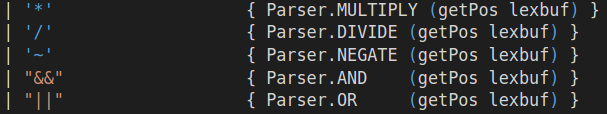
\includegraphics[width=\linewidth]{Materials/Lexer/Lexer}

    \section{Parser}
Once the lexer has recognized input, the parser is in charge of handling said input. For example, if the lexer recognizes an \textit{or}-expression, the parser must determine if the semantics are in order - for example if the \textit{or}-operator is used, it must check if the operator is used on two expressions in a proper maner. If not, the parser must recognize this and a parsing-error will occur. Returning to the \textit{or}-operator, it only makes sense if the \textit{or}-keyword is sandwiched between two expressions or else the use of the \textit{or}-operator doesn't fit its formal definition. The parser checks if this is the case, and if so, calls upon the typechecker to ensure the types of the expressions are in order. The check, which the parser makes, looks like this in our implementation:\\
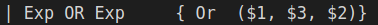
\includegraphics[width=\linewidth]{Materials/Parser/Or}\\
This implementation ensures that only the \textit{or}-operator when sandwiched between two expressions is accepted, or else an error will be raised. 

    \section{Typechecker}
An fs file \textit{TypeChecker.fs} has been implemented, the purpose of which is to ensure that the types, on which arithmetic operators (\textit{plus,minus,etc.}), logical operators (\textit{and,or}) and others, match the given operator.
For example, if we want to implement the \textit{or}-operator, we need to ensure that the operator will only be aplied on boolean values, as any other values don't make sense given the specification of the \textit{or}-operator.\\
The implementation of the typechecker for the \textit{or}-operator, can be seen here: \\
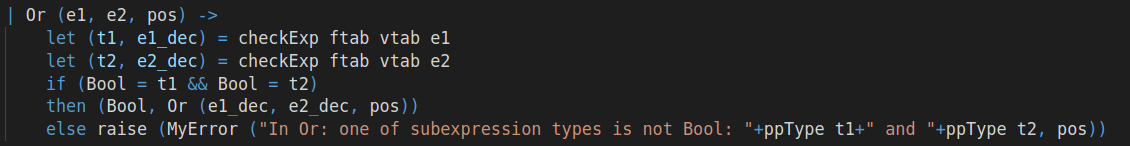
\includegraphics[width=\linewidth]{Materials/TypeChecker/Or}\\
Focusing on the \textit{or}-operator (since other operators are implemented in largely the same way), the typechecking works as follows:\\
First, we call the checkExp function and match with the \textit{Or}-keyword and parse it the two expressions no which we operator and the position.
Afterwards, we determine the type of our expressions by calling the checkExp function whilst supplying it our Function-table and Value-table.\\
Next, we check that both types match (i.e are boolean values). If so, we run theimplemented \textit{or}-function as found in \textit{codeGen.fs} on our expressions, which we now know to be of the type bool. If the \textit{or}-operator is not called on bools, we raise an error stating that at least one of the expressions is of the wrong type.\\
The typechecker works the same for all other operators, except possibly checking on other types like Ints for an arithmetic operator. 

	\section{CodeGen}
\subsection{Filter}
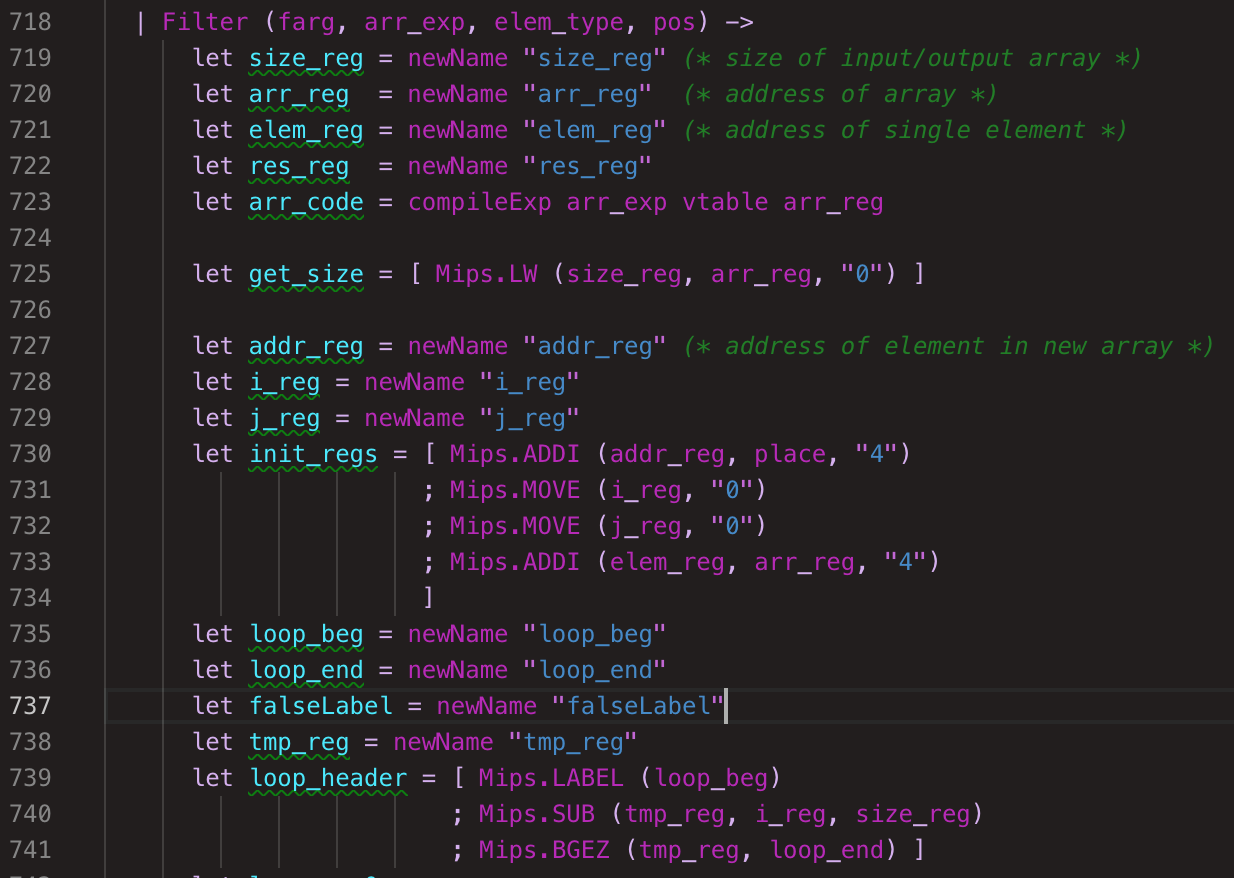
\includegraphics[width=\linewidth]{Materials/CodeGen/filterIntro}
Filter is implemented much like 'map'. To implement filter we first create a new array of the same size as the input array. We also create some new registers to keep track of the memory locations of the elements in the new array (\textit{addr\_reg}) and the input array (\textit{elem\_reg}). Lastly we create a register (\textit{j\_reg}) to count how many elements we have added to the new array.\\
The idea is we create a loop where we apply the input function on the first element of the input array, and if the output is \textit{true} we then add it to the new array, we add to the registers working as pointers to the elements in the array such that we move to the next entry in the arrays and lastly we add one to our counter register \textit{j\_reg}. If the output is \textit{false}, we only add to the \textit{elem\_reg} and then begin the loop anew on the next element of the input array.\\
We do this by loading the value of the input array into \textit{res\_reg} and apply the input function using the helper function \textit{applyFunArg} on lines 742-747.
 
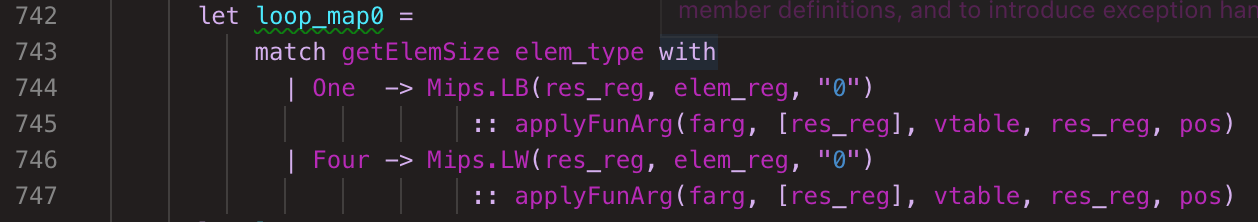
\includegraphics[width=\linewidth]{Materials/CodeGen/filter1}
We now have either '1' or '0' (true, false) in \textit{res\_reg}. We now load the value of \textit{elem\_reg} into a temporary register for use if the result is true. Then we add to \textit{elem\_reg} to have it point to the next entry of the input array. We now do a conditional branching. If the value of \textit{res\_reg} is true, we fall through, else we jump. In the case the result is \textit{true}, we save the value in \textit{tmp\_reg} in \textit{addr\_reg}, we add to \textit{addr\_reg} such that it points to the next entry of the array and we add 1 to \textit{j\_reg}. Then we meet the point where we would jump to if the result had been false (line 762), and the loop begins anew. All of this is done on lines 748-765. When the loop terminates after having iterated over all entries in the input array, we then shrink the size of our new array to its actual size using \textit{j\_reg} on line 766.

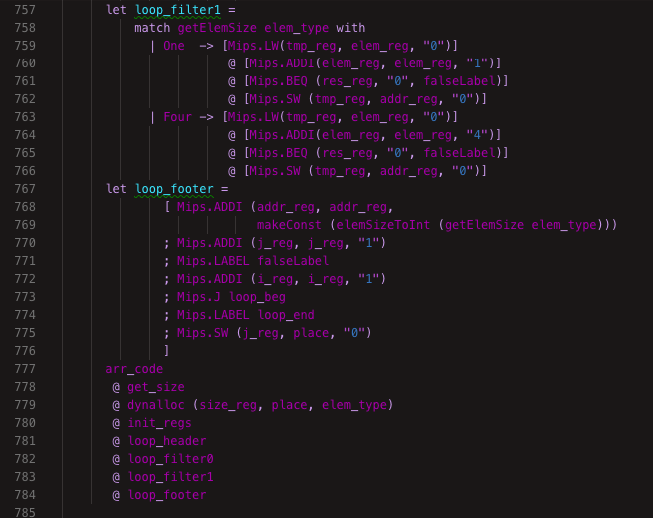
\includegraphics[width=\linewidth]{Materials/CodeGen/filter2}
\subsection{Replicate}
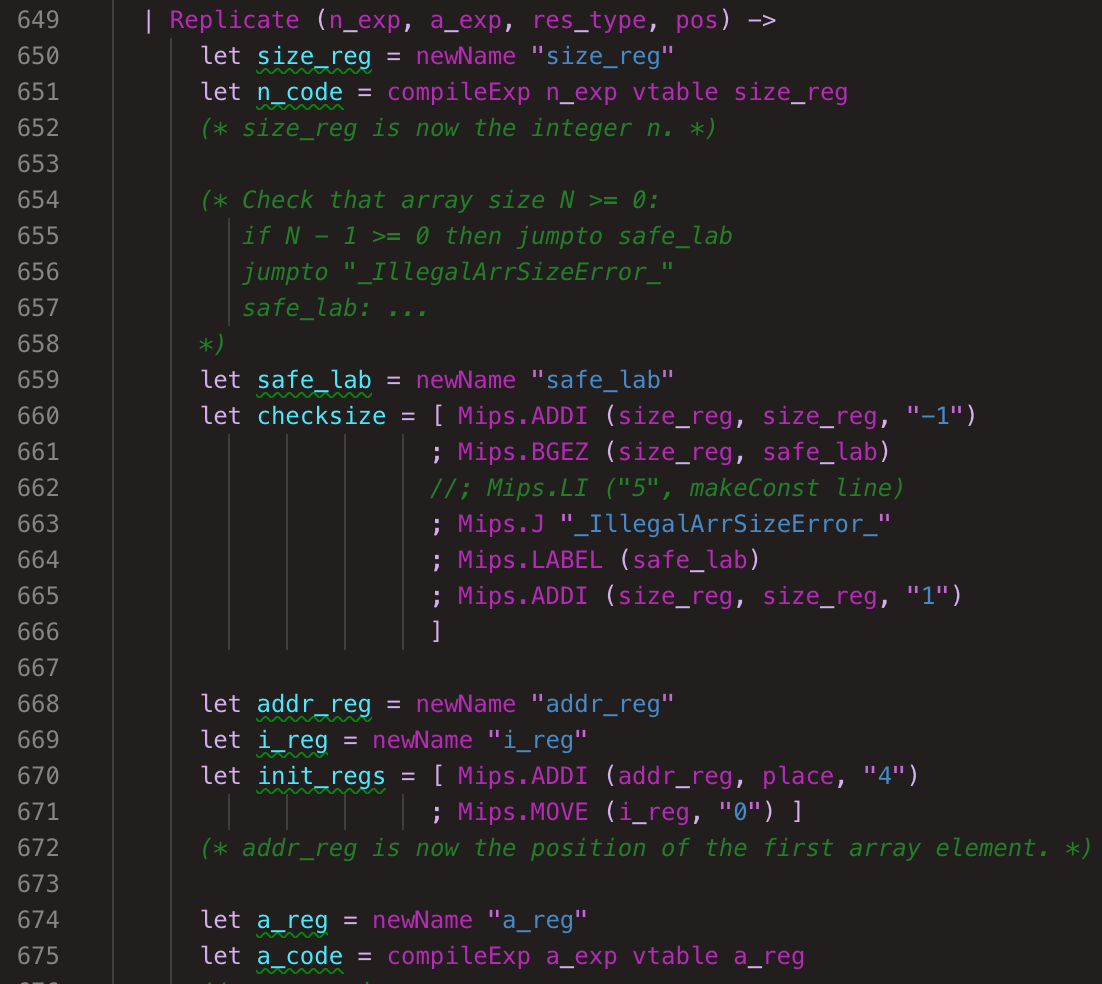
\includegraphics[width=\linewidth]{Materials/CodeGen/ReplicateIntro}
To implement replicate we first check if the given '\textit{n expression}' is greater than zero, and then we create a new array of size \textit{n} (lines 650-666). Then we create a register \textit{addr\_reg} which points to the first entry in the new array and we create another register \textit{a\_reg} which contains our given input which we want to replicate.\\
The idea is we create a loop and in each iteration we put the value of \textit{a\_reg} into the new array.\\
First we save the value of \textit{a\_reg} in \textit{addr\_reg} such that the entry in the new array which \textit{addr\_reg} points to now contains the replicated value. Then we add to \textit{addr\_reg} so it points to the next entry and we update the loop counter \textit{i\_reg} and start the loop anew. All of this is done on lines 680-693.\\
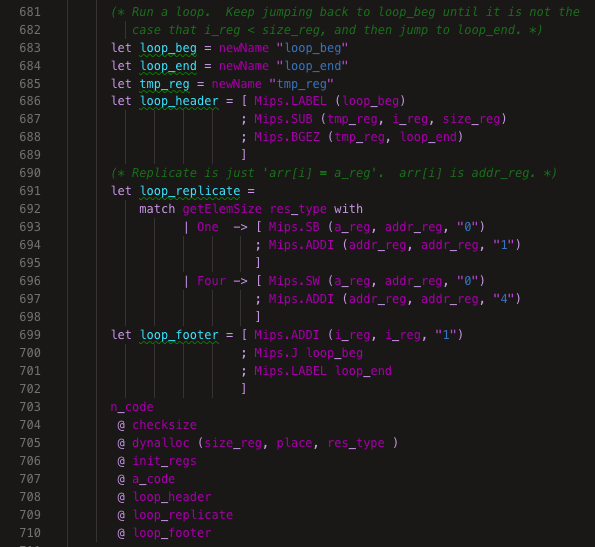
\includegraphics[width=\linewidth]{Materials/CodeGen/Replicate1}

\subsection{Scan}
The idea is we create a register to hold the accumulated value. Then we create a loop in where we apply the supplied function on the value in the accumulated register and the element in the input array and we save the value in the accumulated register. Then we save the value in the accumulated register in the new array and we begin the loop anew.
	\section{Interpreter}
For \textit{Times, Divide, And, Or, Not} and \textit{Negate} the general idea is to first evaluate the expressions, and then pattern match the resulting expressions' type. If successful then return the result, otherwise we throw an error. For \textit{And} and \textit{Or} we have nested pattern matching in order to achieve short circuiting. This is all implemented on lines 165 - 207 of Interpreter.fs.\\
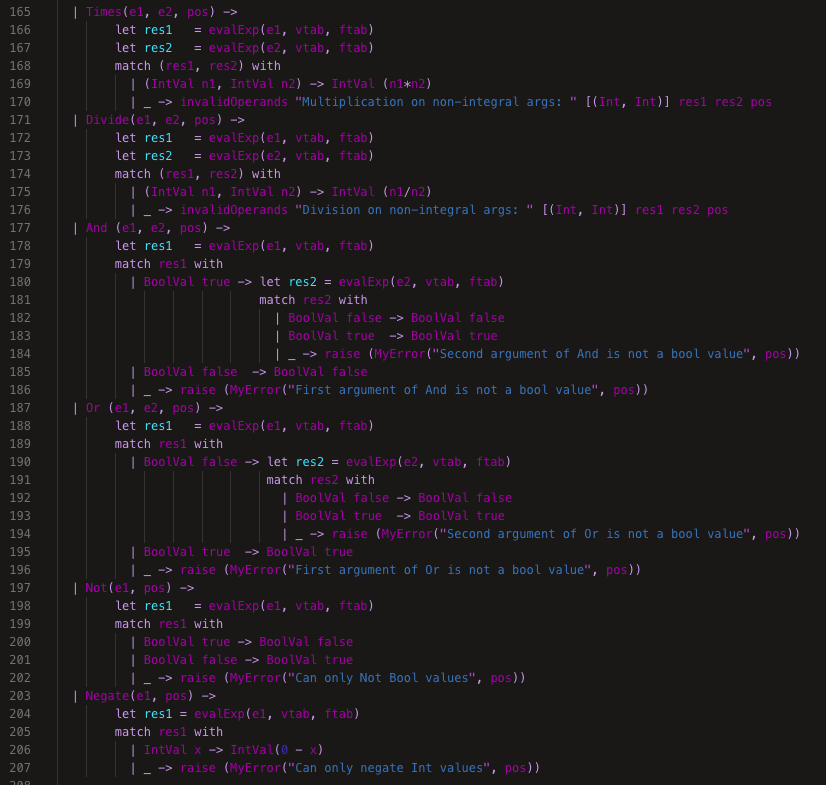
\includegraphics[width=\linewidth]{Materials/Interpreter/Expressions}\\
The functions are implemented somewhat similarly by first evaluating the expressions and then match the resulting expressions' types.\\
Replicate pattern matches for its first argument being of type int and being grater or equal to zero and for the second argument to be of type int, bool or char. If it succeeds it uses the f\# function 'List.replicate' to construct the output. (lines 300 - 308).\\
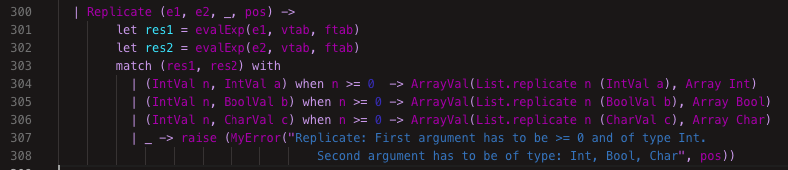
\includegraphics[width=\linewidth]{Materials/Interpreter/Replicate}\\
Filter matches its second argument with an array. If it succeeds it uses the f\# function 'List.filter' to create the output. But to make sure the first argument return bool, a lambda expression is passed to List.filter which pattern matches the output of the function passed to Filter with bool values. (lines 319 - 333).\\
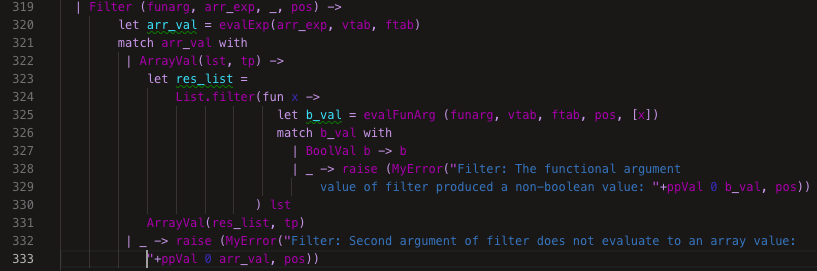
\includegraphics[width=\linewidth]{Materials/Interpreter/Filter}\\
Scan works similarly as the previous functions, as it pattern matches an array and if it succeeds it uses the f\# function 'List.scan' to construct the output. (lines 339 - 347).\\
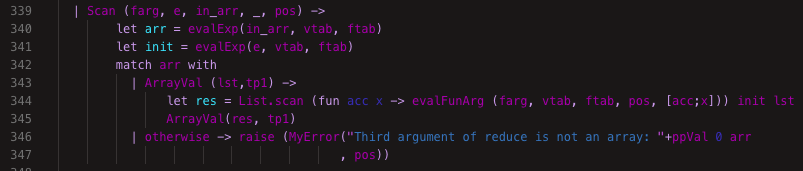
\includegraphics[width=\linewidth]{Materials/Interpreter/Scan}\\
        \section{multilet}
Multilet has been implemented like so:\\
First off, implement the lexer as to recognize semicolons like so:\\
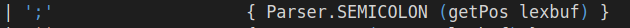
\includegraphics[width=\linewidth]{Materials/Lexer/MultiletLexer}
When the lexer recognizes the semicolon, it parses it to the parser and matches it with the following statement:\\
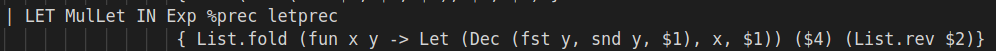
\includegraphics[width=\linewidth]{Materials/Parser/MultiletMatch}
The definition of multlet is given in the following, recursive function:\\
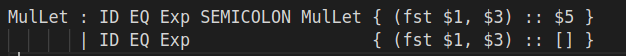
\includegraphics[width=\linewidth]{Materials/Parser/MultiletParser}\\
This function adds the given ID and Expression to a list. If a semicolon is met, the function is called again as there are more let-bindings to add to the list. If no semicolon is met, the ID and expression is added to an empty list as to stop the recursive calls since there are no more let-bindings to be made and the next keyword is expected to be IN. Afterwards, we call our let-function on each element in the list. When finished, we have succesfully bounded multiple IDs with multiple expressions.  

	\section{Optimization}
\subsection{CopyConstPropFold.fs}
The optimization done in 'copyConstPropFold.fs' revolves around substituting longer abstract syntax tree expressions with smaller more optimized abstract syntax tree expressions. For instance, a long expression involving multiplication with zero will always result in zero, and thus as soon we see we are doing multiplication with zero we can just return the optimized expression zero. This optimization along with optimization for multiplication with one has been implemented on lines 85-97 in CopyConstPropFold.fs as seen below.\\
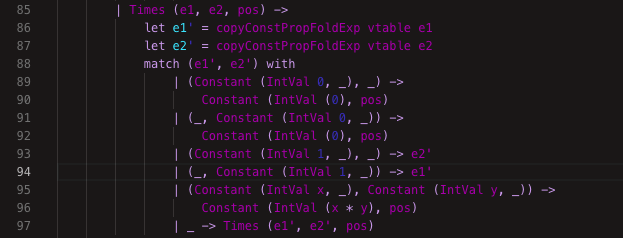
\includegraphics[width=\linewidth]{Materials/Optimization/Times}\\
Similarly short circuiting has been implemented on lines 98-107 for \textit{And}.\\
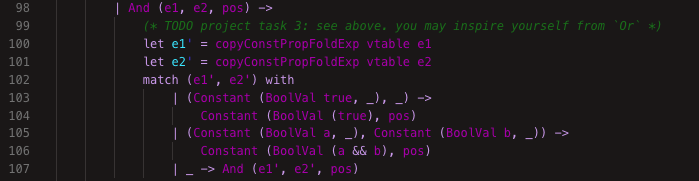
\includegraphics[width=\linewidth]{Materials/Optimization/And}\\
Following the instructions in the lecture slides\footnote{Lecture slides, 9-Optim-Fasto.pdf} the cases for \textit{Var, Index} and \textit{Let bindings} has been implemented. In the case of \textit{Var} we look in the symbol table for the variable, if it exists we replace it with an abstract syntax tree of its value, otherwise we do nothing. For the \textit{Index} case we attempt to optimize the expression and then look up the name of the array in the symbol table. If the name exists we replace the former abstract syntax tree with a new one constructed as the new name and the optimized expression. Otherwise we construct a new 'Index' abstract syntax tree with the old name and the optimized expression (lines 24-45 in CopyConstPropFold.fs).\\
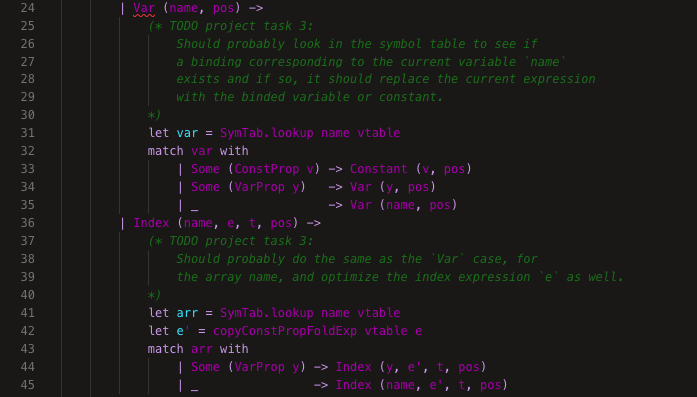
\includegraphics[width=\linewidth]{Materials/Optimization/VarIndex}\\
The last case \textit{Let} can be split into another three cases: \textit{Var, Constant} and \textit{Let}. In all cases the expression is always optimized.\\
In the case of \textit{Var}, a binding of the outer \textit{Let} name is made with the variable and added to the symbol table. The outer \textit{Let} body is then attempted optimized according to this new symbol table. And lastly a new 'Let' abstract syntax tree is constructed with the outer \textit{Let} name, the optimized expression and the optimized outer \textit{Let} body. Similarly is done for \textit{Constant}. If we reach the \textit{Let} case we rearrange the let bindings such that they get optimized and we run \textit{copyConstPropFoldExp} to optimize this new expression. All of this is done on lines 46-81 of CopyConstPropFold.fs.\\
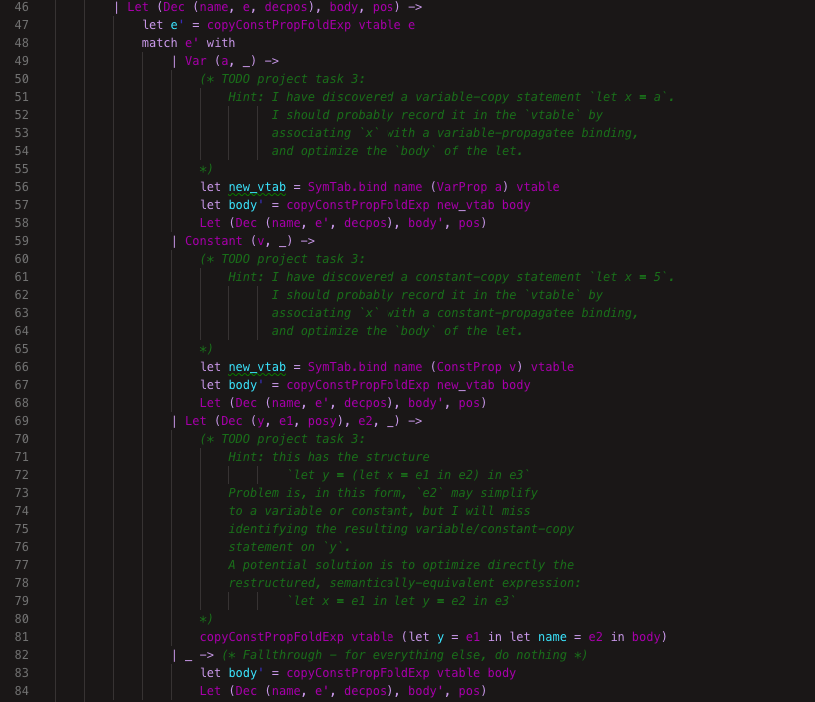
\includegraphics[width=\linewidth]{Materials/Optimization/Let}
\subsection{DeadBindingRemoval.fs}
Following the instructions in the lecture slides\footnote{Lecture slides, 9-Optim-Fasto.pdf} dead binding elimination has been implemented. In the case of \textit{Var} we know there will not be any IO, and we can not optimize the abstract syntax tree. Thus we construct a triple tuple of \textit{false} for IO, an empty symbol table with the variable name appended and 'Var (name, pos)'. (lines 63 - 70 of DeadBindingRemoval.fs).\\
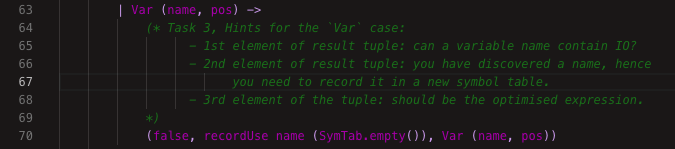
\includegraphics[width=\linewidth]{Materials/Optimization/VarDBE}\\
For \textit{Index} we recursively optimize the expression and return the results thereof. (lines 72 - 79).\\
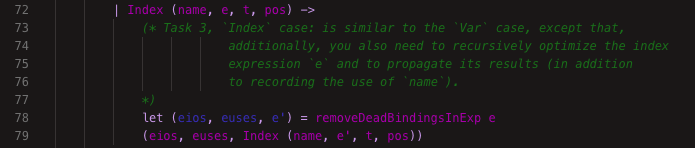
\includegraphics[width=\linewidth]{Materials/Optimization/IndexDBE}\\
For \textit{Let} we recursively optimize the body and the expression. We now optimize based on whether we can remove the expression or not. (lines 81 - 102).\\
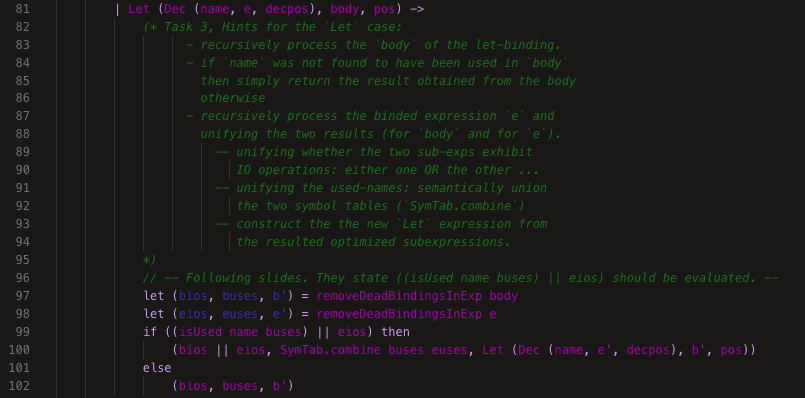
\includegraphics[width=\linewidth]{Materials/Optimization/LetDBE}\\
Dead binding elimination is done similarly for all other expressions.


        \section{Tests}
Several tests have been included in our assignment to test the functionality of our implemented functions. Also, new ones have been created to further test the functionality of our fasto-compiler.\\
For example, we have written the following test for the functionality of the \textit{or}-operator, which looks as so:\\
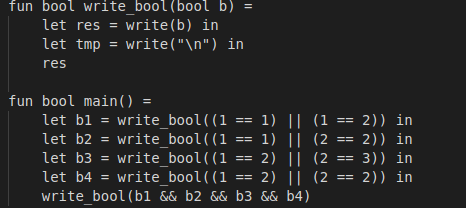
\includegraphics[width=\linewidth]{Materials/Tests/OrTest}
This test (alongside most others) suceed by matching expected input. In the case of the test above, the expected output, which it matches, looks like the following:\\
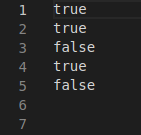
\includegraphics[width=0.4\linewidth]{Materials/Tests/OrExpected}\\
Some tests have been made only to test the typechecker.These tests purposefully use nonsensical types (like using the \textit{or}-operator between integers or multiplying an int with a bool). The typechecker-test with regards to the \textit{or}-operator looks like so:\\
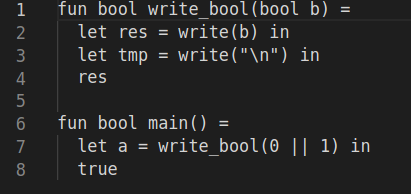
\includegraphics[width=\linewidth]{Materials/Tests/OrTypeCheck}\\
The test succeeds as the accompanying \textit{.err}-file expects the appropriate error-message reflecting the error. In this case, the error is a type-missmatch, as the \textit{or}-operator expects two bools but is given two integers instead. Also, this test doubles as a reassurence that $0$ and $1$ aren't evaluated as \textit{false} and \textit{true}, respectively. 

\end{document}
